\chapter{IP伝送装置の技術要件}
\label{chap:video-technology}

本章では、映像伝送システムを構成する技術要素とその仕組みについて解説する。また、本研究でIP伝送装置を実装するにあたり、技術要件をまとめる。

\section{ビデオカメラ}
\label{sec:camera}

% ここはaomさんの引用なので適切にする
ビデオカメラは、映像の入力機構である。
撮影素子であるイメージセンサは、多数の受光素子によって構成されており、それぞれの受光素子は、光エネルギーの明暗に従い電荷を発生する。
撮影対象部から反射される光をカメラのレンズを通して、この撮影素子の受光部にあてることで、その明暗を電荷量を光電変換する。
変換された電圧値を順次読み出し,電気信号に変換することでアナログ値である光情報をデジタル値に変換する。

ビデオカメラによる出力インターフェースとしては、デジタル信号としてはSDIやHDMIのインターフェースを使用するのが一般的である。

\section{ディスプレイ}
\label{sec:display}

% ここはaomさんの引用なので適切にする
ディスプレイは、映像の表示機構である。
ディスプレイには大まかに、アナログディスプレイとデジタルディスプレイに二分できる。

アナログディスプレイでは、CRT、すなわちブラウン管を用いた描画方式である。
管面全体を走査線とよぶ固定パターンでスキャンしつつ、映像信号の輝度成分に従って電子ビームの強さを変調して描画する。
このように、画面上の任意の点の明るさを制御することにより画像を作り上げている。

一方、デジタルディスプレイでは、薄い板状の液晶パネルを用いた描画方式である。
偏光フィルタから入ってきた光を、電極によりピクセルのカラーごとに電荷をかけることにより、配向膜を光が通り抜け描画する。
ブ゙ラウン管の走査方式を後継しており、映像の制御信号として、水平同期信号と垂直同期信号が使われている。

\section{インターレース}
\label{sec:interlace}

画像伝送において、データレートを増やさずに描画回数を増やす技術である。
この方式の特徴は、「人間の視野は動くものの細部を捉えられない」という性質に基づいている。
飛び越し走査とも呼ばれ、奇数番目の走査線を先に送り、偶数番目の走査線をその後に送る。

デジタル化が進んでいる現在でも、走査線を1ラインに割り当て、データレートを減らす際の手段として利用されている。
また、インターレースではない、画像をプログレッシブと呼び、インターレースからプログレッシブに変換する処理を、デインターレースと呼ぶ。
% 一時停止をした際に、動きの激しい箇所が
% デインターレースにはいくつかの方式があり、
% 縞模様

主な例として、日本のテレビジョン放送では、アナログテレビ放送、デジタルテレビ放送のどちらでも使われている。
幸いなことに、4K・8K映像ではインターレース方式は使われることはない。% [要出典]
% 幸いな理由と出典先を明示する

\section{色空間と色深度}
\label{sec:colorspace}

一般的に液晶ディスプレイでは、1ピクセルを赤、緑、青、すなわちRGBの3つの色信号で表現する。
多くのPCやゲーム機の出力ではRGBの色空間が使われ、RGBそれぞれ8bit、1ピクセルあたり24bitで表現する。
1ピクセルあたりを表現するビット数を色深度といい、色解像度、色分解能とも言われる。
24bitの色深度では、16,777,216色を表現することができる。

一方、ビデオカメラでは、輝度信号Yと2つの色差信号を使って表現される色空間であるYUVが使われることが多い。% [要出典]
この方式の特徴は、「人間の目は明るさの変化には敏感だが、色の変化には鈍感である」という性質に基づいて、色度信号の情報量を減らすことができるという点にある。

\begin{figure}[htbp]
  \begin{center}
    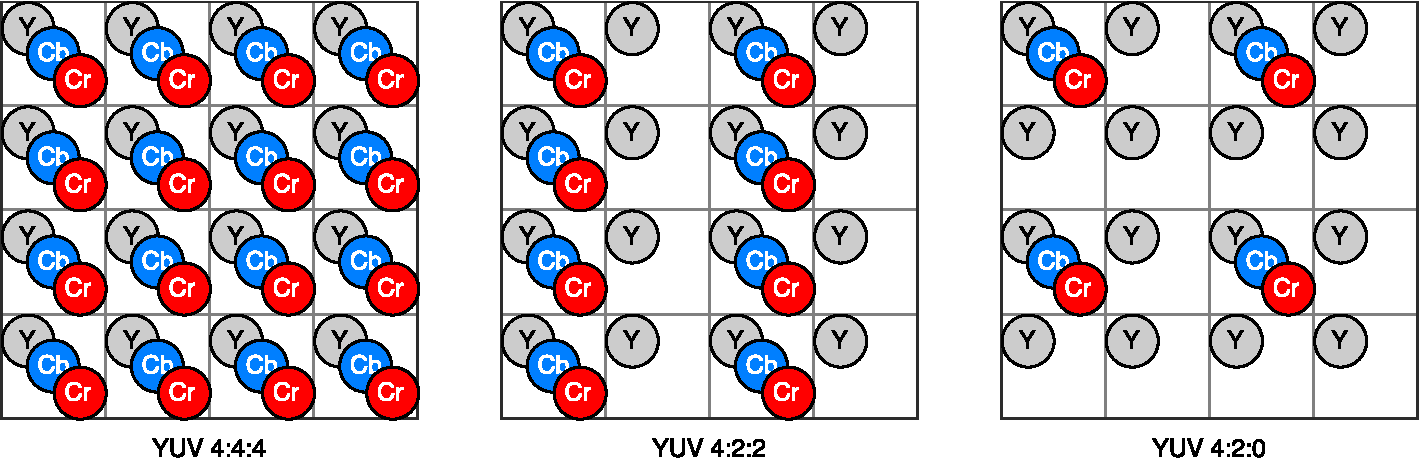
\includegraphics[bb=0 0 681 222,width=14cm]{img/yuv-pixel-structure.pdf}
  \end{center}
  \caption{YUVのピクセルあたりの色情報の構造}
  \label{fig:yuv-pixel-structure}
\end{figure}

% YUVのピクセルあたりの色情報の構造を、図\ref{fig:yuv-pixel-structure}に示す。

YUV 4:4:4では、輝度信号、色差信号共に1ピクセル毎である。
YUV 4:2:2では、輝度信号は1ピクセル毎、色差信号は2ピクセル毎であり、同じ色深度のYUV 4:4:4と比べ、帯域はおよそ2/3となる。
YUV 4:2:0では、輝度信号は1ピクセル毎、色差信号は4ピクセル毎であり、同じ色深度のYUV 4:2:2と比べ、帯域はおよそ3/4となり、同じ色深度のYUV 4:4:4と比べ、帯域はおよそ1/2となる。

なお、図\ref{fig:yuv-pixel-structure}で示した、UV成分であるCb、Crの色のサンプリング方法は、伝送方式の規格によって定められている。

\section{インターフェース}
\label{sec:interface}

\subsection{VGA}
VGA(Video Graphics Array)は、IBMが発表したアナログ映像信号の伝送規格、または、同社が開発したVGA表示回路用のチップのことを指す。
DE-15コネクタを使用し、赤、緑、青、垂直同期、水平同期の5つのアナログ信号で映像を伝送することができる。
DDC(VESA Display Data Channel)信号を使用することで、接続機器の対応する解像度を送信することができ、最近では1080pの映像を伝送する機器も多い。
PCでの映像出力方式として普及したが、アナログ信号であることや、音声伝送の手段が別途必要となるため、HDMIやDisplayPortなどのインターフェースに移行が進んでいる。

\subsection{DisplayPort}
DisplayPortは、VESA\footnote{Video Electronics Standards Association ビデオ周辺機器に関する業界標準化団体}によって標準化された映像伝送規格であり、主に超解像度向けのインターフェースとして普及している。
DisplayPort 1.3からは、32.4 Gbpsのデータレートに対応し、8K映像の伝送にも対応している。

\subsection{DVI}
DVI(Digital Visual Interface)は、VESA\footnotemark[1]によって標準化された デジタル映像信号の伝送規格である。
物理層として、Silicon Imageが開発したTMDS(Transition Minimized Differential Signaling)を使用している。
TMDSは、データの3チャネルとクロックの1チャネルを備えた4つのツイストペアケーブルで構成され、主に高速シリアル通信で使用されている。
TMDSでは、データの8b/10b符号化が行われ、データレートは20\%のロスとなるが、DC成分の偏りを押さえ、ブランキング区間などでもI/Oの遷移を増やしてデータの境界検出を用意にしている。

\subsection{HDMI}
HDMI(High-Definition Multimedia Interface)は、映像、音声をデジタル信号で伝送する通信インターフェースの規格である。
DVIを基に、音声伝送機能や著作権保護機能を加えたものであり、物理層はDVIと同じTMDSを使用している。

HDMIのシステム構成は大きく分けて、映像を送る機器(Source)、映像を受け取る機器(Sink)、ケーブルの3つに分類することができる。

\begin{figure}[htbp]
  \begin{center}
    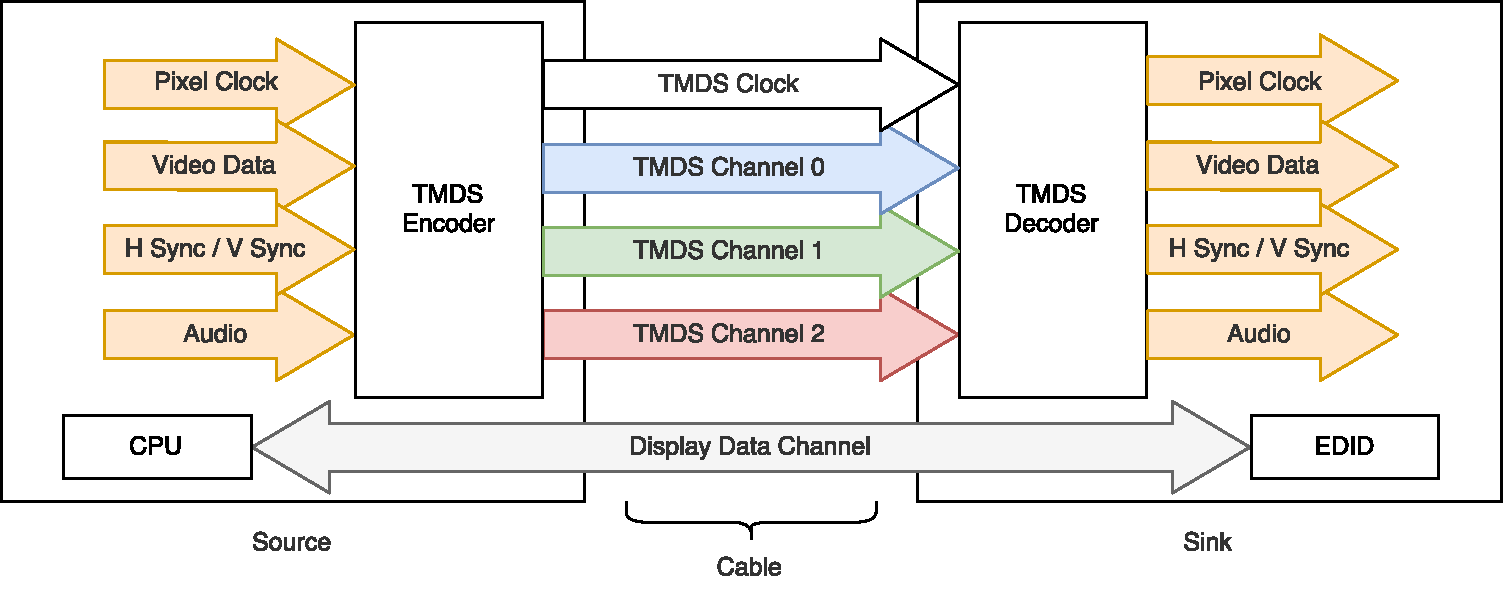
\includegraphics[bb=0 0 721 283,width=15cm]{img/hdmi-spec-structure.pdf}
  \end{center}
  \caption{HDMIブロックダイアグラム}
  \label{fig:hdmi-spec-structure}
\end{figure}

HDMI 2.0では、帯域を18Gbpsに拡大し、4K@60pに対応している。
また、CES 2017に合わせ、HDMI 2.1が発表され、帯域を48Gbpsに拡大し、8K@60pに対応した。

\begin{table}[htbp]
  \caption{HDMI 1.4と2.0での4K(3840x2160)映像の対応状況}
  \label{tb:video-bandwidth}
  \begin{center}
  \begin{tabular}{c|c|c|c}
    \hline
      フレームレート & ピクセルあたりの色深度 & HDMI 1.4 & HDMI 2.0\\\hline\hline
    \multirow{4}{*}{30Hz} &
        24bit & 対応   & 対応 \\\cline{2-4}
      & 30bit & 対応   & 対応 \\\cline{2-4}
      & 36bit & 対応   & 対応 \\\cline{2-4}
      & 48bit & 非対応 & 対応 \\\hline
    \multirow{4}{*}{60Hz} &
        24bit & 非対応 & 対応  \\\cline{2-4}
      & 30bit & 非対応 & 対応  \\\cline{2-4}
      & 36bit & 非対応 & 対応  \\\cline{2-4}
      & 48bit & 非対応 & 非対応 \\\hline
  \end{tabular}\end{center}
\end{table}

HDMI 1.4\cite{hdmi-spec-1-4}では、RGB、YCbCr 4:4:4、YCbCr 4:2:2の色空間がサポートされている。
HDMI 2.0\cite{hdmi-spec-2-0}では、4K解像度向けにYCbCr 4:2:0の色空間がサポートされた。
YCbCr 4:2:0によるピクセルエンコーディングの規格では、YCbCr 4:2:2と比べ、1/2のデータレートで転送することが可能となった。
これにより、一部の機器では4K解像度への対応をソフトウェアだけで行なうことが可能である。

YCbCr 4:4:4、YCbCr 4:2:2のTMDSデータのマッピングを、図\ref{fig:hdmi-spec-yuv-444}と図\ref{fig:hdmi-spec-yuv-422}に示す。

\begin{figure}[htbp]
  \begin{center}
    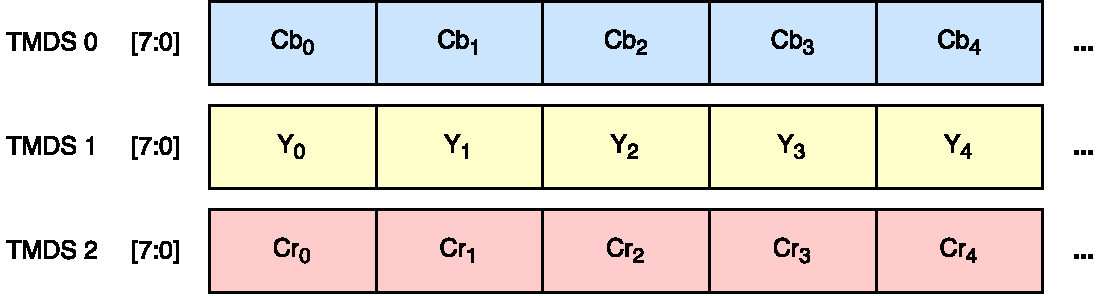
\includegraphics[bb=0 0 531 141,width=13.926cm]{img/hdmi-spec-yuv-444.pdf}
  \end{center}
  \caption{HDMI 1.4 で定義されている YCbCr 4:4:4 におけるTMDSマッピング}
  \label{fig:hdmi-spec-yuv-444}
\end{figure}

\begin{figure}[htbp]
  \begin{center}
    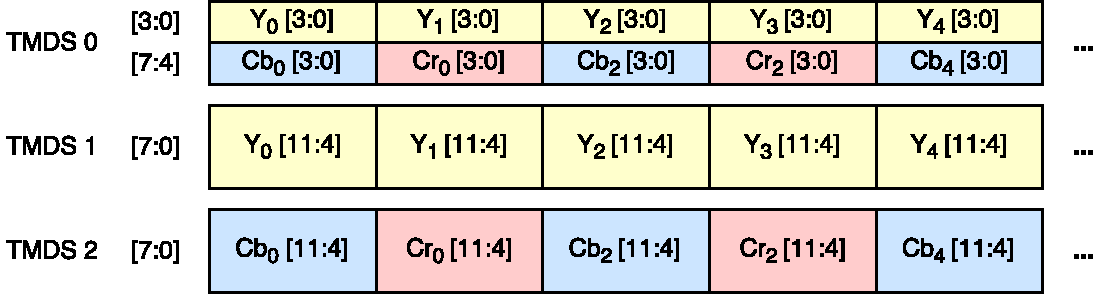
\includegraphics[bb=0 0 531 141,width=13.926cm]{img/hdmi-spec-yuv-422.pdf}
  \end{center}
  \caption{HDMI 1.4 で定義されている YCbCr 4:2:2 におけるTMDSマッピング}
  \label{fig:hdmi-spec-yuv-422}
\end{figure}

\ref{sec:colorspace}節では、同じ色深度の場合YUV 4:2:2はYUV 4:4:4と比べ帯域が2/3になると述べたが、HDMI 1.4で定義されているYCbCr 4:2:2では、1ピクセルあたりの色深度は変わらず、YおよびCbCrのサンプリング解像度が8bitから12bitになる。
そのため、HDMIでは色空間のYCbCr 4:4:4、YCbCr 4:2:2のどちらであっても帯域には影響しない。

\newpage
YCbCr 4:2:0のTMDSデータのマッピングを、図\ref{fig:hdmi-spec-yuv-420}に示す。

\begin{figure}[htbp]
  \begin{center}
    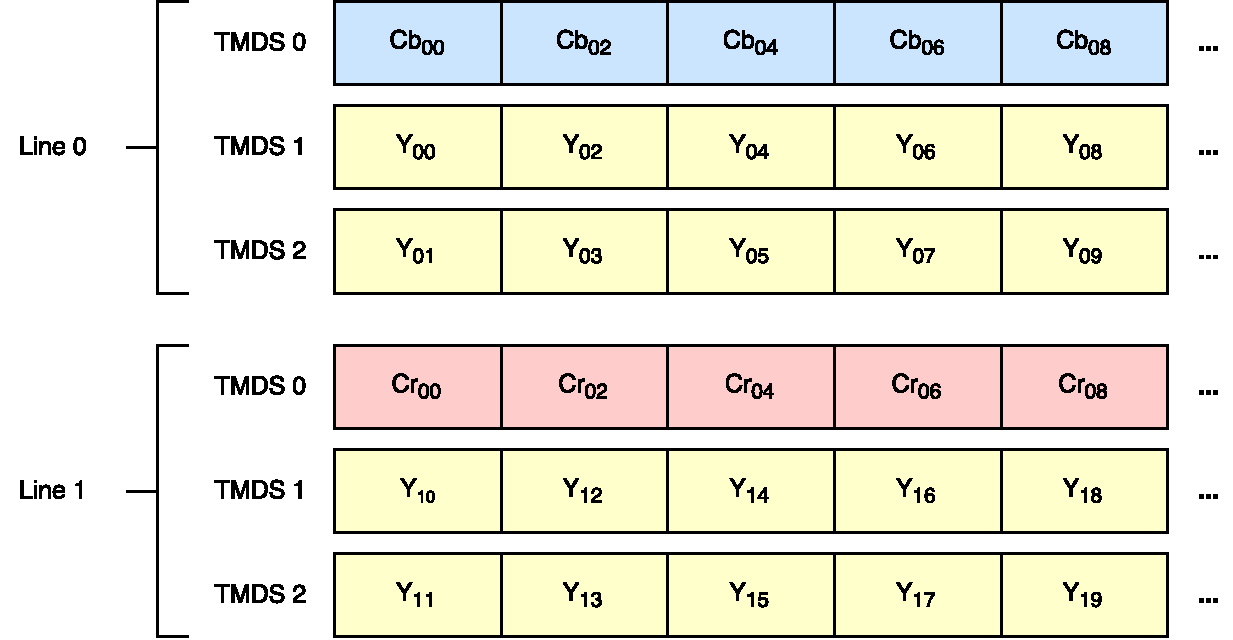
\includegraphics[bb=0 0 591 306,width=15.5cm]{img/hdmi-spec-yuv-420.pdf}
  \end{center}
  \caption{HDMI 2.0 で定義されている YCbCr 4:2:0 におけるTMDSマッピング}
  \label{fig:hdmi-spec-yuv-420}
\end{figure}

HDMIでは、24bitの他に、30bit、36bit、48bitの色深度に対応しているが、YCbCr 4:2:0では、24bitのみの対応である。

\subsection{SDI}

SDI(Serial Digital Interface)は、SMPTE\footnote{米国映画テレビ技術者協会}によって標準化された映像伝送規格であり、主に業務機器向けの規格である。

同軸ケーブルを使用しているため、HDMIと比べて距離に対する減衰が少なく、HD-SDIでは、およそ100m遠方に伝送することができる。
BNC端子を使用することが一般的であり、抜け落ち防止のためのロック機能がるため、放送局や中継現場で使われる。

解像度や帯域に応じて、SD-SDI、HD-SDI、3G-SDI、6G-SDI、12G-SDIなど複数の規格が定められている。
また、4K・8K映像を伝送するために、HD-SDIや3G-SDIを2本1組や4本1組で使用して伝送する規格も定められている。

\section{帯域}
\label{sec:bandwidth}
帯域は解像度の他にも、インターレース、色空間、色深度により変化する。
また、伝送するインターフェースの規格によっても、物理層での扱いにより若干の違いがある。
ここでは、HDMIで色深度を8bitとした場合の解像度、フレームレート、色空間別に見たピクセルクロック、データレートを表\ref{tb:video-bandwidth}に示す。

% 1920x1080p/60 2200x1125 148.5 SMPTE 274M
% 1Channel = 2200 * 1125 * 3 * 8 * 60 * 1.25/3

同期区間を含めた垂直ピクセルを$p_w$、水平ピクセルを$p_h$、ピクセルあたりのビット数を$b$、フレームレートを$f$としたとき、HDMIのデータレート$r$は次のようにして求めることができる。
HDMIの物理層であるTMDSでは、8b/10b変換が行われるため、データレートとしては1.25倍となることに注意していただきたい。

\[ r=1.25bfp_wp_h \]

\begin{table}[htbp]
  \caption{解像度、フレームレート、色空間によるHDMIのデータレートの変化}
  \label{tb:video-bandwidth}
  \begin{center}
  \begin{tabular}{c|c|c|c|c}
    \hline
    解像度     & フレームレート & 色空間  & ピクセルクロック & データレート  \\\hline\hline
    3840x2160 & 60p          & RGB    & 594MHz        & 17.82 Gbps  \\\hline
    3840x2160 & 60p          & YUV422 & 594MHz        & 17.82 Gbps  \\\hline
    3840x2160 & 60p          & YUV420 & 297MHz        & 8.91 Gbps   \\\hline
    3840x2160 & 30p          & RGB    & 297MHz        & 8.91 Gbps   \\\hline
    3840x2160 & 30p          & YUV422 & 297MHz        & 8.91 Gbps   \\\hline
    1920x1080 & 60p          & RGB    & 148.5MHz      & 4.455 Gbps  \\\hline
    1920x1080 & 60p          & YUV422 & 148.5MHz      & 4.455 Gbps  \\\hline
    1920x1080 & 60i          & RGB    & 74.25MHz      & 2.2275 Gbps \\\hline
    1920x1080 & 60i          & YUV422 & 74.25MHz      & 2.2275 Gbps \\\hline
  \end{tabular}\end{center}
\end{table}

\section{IP伝送規格}
Video over IPにおける映像のIP伝送規格は、SMPTE 2022とNMIが主流となっている\cite{kodera-interbee2016}。
しかし、その他にも多くの規格が提唱され、市場ではどの規格で統一されるかが静観されている。

IP伝送規格は、SDIなどの標準化を行っているSMPTEや、映像制作現場などの機器を制作している会社が製品とともに規格化を行う事が多い。
この節では、抜粋して幾つかのIP伝送規格について解説する。

\subsection{SMPTE 2022}
SMPTE 2022は、SMPTEが提唱、標準化したIP伝送規格であり、表\ref{tb:smpte2022-abstract}に示す7つの規格に分かれている。

\begin{table}[htbp]
  \caption{SMPTE 2022の7つの規格の概要}
  \label{tb:smpte2022-abstract}
  \begin{center}
  \begin{tabular}{c|l}
    \hline
    規格          & 概要 \\\hline\hline
    SMPTE 2022-1 & IP伝送でのリアルタイムビデオ/オーディオ転送のFEC訂正 \\\hline
    SMPTE 2022-2 & IP伝送での固定ビットレートMPEG-2 TSの単方向転送 \\\hline
    SMPTE 2022-3 & IP伝送での可変ビットレートMPEG-2 TSの単方向転送 \\\hline
    SMPTE 2022-4 & IP伝送での非ピース単位の可変ビットレートMPEG-2ストリームの単方向転送 \\\hline
    SMPTE 2022-5 & IP伝送での高ビットレートメディア信号の伝送のための前方誤り訂正 \\\hline
    SMPTE 2022-6 & IP伝送でのネットワークを介した高ビットレートメディア信号の伝送 \\\hline
    SMPTE 2022-7 & IPデータグラムのシームレスな保護スイッチング \\\hline
  \end{tabular}\end{center}
\end{table}

SMPTE 2022-1/2/3/4では、MPEG2圧縮をベースとしたIP伝送について規格化され、SMPTE 2022-5/6では、非圧縮でありSDIのペイロードを基としたIP伝送について規格化されている。

\subsection{SMPTE 2110}
SMPTE 2110は、SMPTEが制定中の規格であり、VSF(Video Services Forum)に提出されたTR03、TR04の内容を取り込んでいる。

SMPTE 2022-5/6ではSDIのペイロードを基としているため、IPパケットにする際にはSDIをカプセル化している。
そのため、映像と音声データをIPレイヤーから識別することができず、制御に利用しにくいなどの問題がある。
この問題を回避するため、SMPTE 2110では、ビデオデータの伝送にはRFC 4175\cite{rfc4175}のRTP、音声データの伝送にはAES 67を使用するなど、より効果的なIP伝送規格になるよう設計されている。

\subsection{NMI ネットワーク・メディア・インターフェース}
NMI\cite{sony-nmi}は、ソニービジネスソリューションが提唱、規格化したIP伝送規格である。

非圧縮ではなく、低遅延高画質のコーデックであり、Visually LosslessなLLVC\cite{smpte-rdd-34}によって圧縮されている。
また、機器間の同期にはナノ秒レベルの高精度同期が行える、SMPTE ST2059を使用している。

\subsection{NDI ネットワーク・デジタル・インターフェース}
NDI\cite{newtek-ndi}は、NewTekが提唱、開発したオープンなIP伝送規格である。

多くのIP伝送規格は商用向けであり、詳細な仕様はオープンになっていないが、NDIではSDKやプラグインなどを公開し、ユーザーを集めている。
同社ではIPワークフローとして、NDIを利用したスイッチャーや入出力システムなどを提供している。

\section{まとめ}
本章では、IP伝送装置における技術要素について解説した。

映像制作現場では、インターフェースとしてSDIが用いられることが多い。
しかし、SDIをインターフェースとする開発環境を整えるためには、コストが問題となる。
そのため、本実装ではコストをより押さえつつ、映像制作現場でも使われているHDMIをインターフェースとする。

計算上では、10Gbpsの帯域で4K 30Pの映像でけでなく、色空間と色深度をYCbCr 4:2:0とすることで4K 60Pの映像も伝送することが可能であった。
本実装では、4K 30Pの他に、YCbCr 4:2:0方式で4K 60Pの映像が伝送できることを要件とする。

IP伝送規格については、SMPTE 2022とNMIが主流であったが、どちらもオープンな規格ではなく規格に沿った実装をすることは困難である。
そのため、今回の実装では独自方式のプロトコルを用いる。

\begin{table}[htbp]
  \caption{IP伝送装置の技術要件}
  \label{tb:ip-youken}
  \begin{center}
  \begin{tabular}{l|l}
    \hline
    インターフェース   & HDMI \\\hline
    \multirow{2}{*}{対応解像度} & 4K 3840x2160 30P \\\cline{2-2}
                              & 4K 3840x2160 60P(但しYCbCr 4:2:0方式)  \\\hline
    プロトコル        & 独自規格 \\\hline
  \end{tabular}\end{center}
\end{table}
